\begin{figure*}[t]
\centering
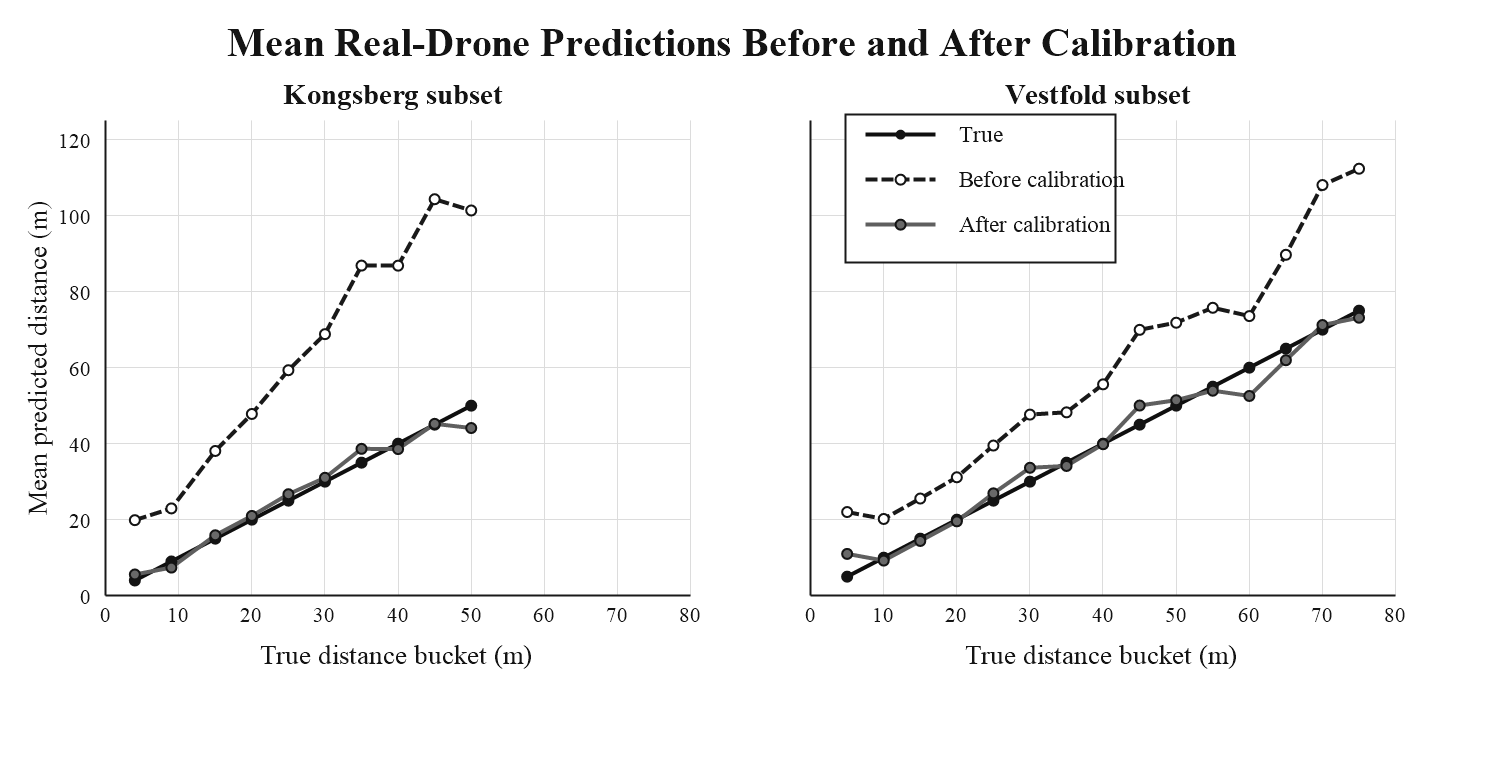
\includegraphics[width=\textwidth]{Sections/Images/fig6.png}
\caption{Mean predicted distance before and after calibration on real drone images. Before calibration, the prediction curve follows the distance trend but remains shifted above the true-distance curve. After calibration, the prediction curve aligns much more closely with the ground truth, showing that calibration removes most of the systematic real-world bias.}
\label{fig:real_calibration_scatter}
\end{figure*}
